\RequirePackage{fixltx2e} %This package in CTeX is not compatible with revtex4-1
\documentclass[aps,pre,12pt,preprint,onecolumn,showpacs,showkeys]{revtex4-1}
\usepackage{ctex}
\usepackage{mathtools}
\usepackage{multirow}
\usepackage{setspace,dcolumn}
\usepackage{subfig}
\usepackage{hyperref}
\usepackage{graphicx,psfrag,epsfig}
\usepackage[font=small,format=plain,labelfont=bf,textfont=it,justification=centering,singlelinecheck=false]{caption}
\usepackage{amsmath,amsfonts,amssymb,amsthm,bm,upgreek}
\usepackage{geometry}
\usepackage[mathscr]{eucal}
\hypersetup{colorlinks=true}
\geometry{top=2.54cm,bottom=2.54cm,left=3cm,right=3cm}
\renewcommand\appendixname{附录}
\renewcommand\abstractname{}%摘要
\renewcommand\tablename{表}
\renewcommand\figurename{图}
\makeatletter
\def\@pacs@name{\songti\zihao{-4}{\bf PACS码:}}
\def\@keys@name{\songti\zihao{-4}{\bf 关键词:}}
\def\Dated@name{日期:}
\def\Received@name{\zihao{-5}{接收} }
\def\Revised@name{\zihao{-5}{修订} }
\def\Accepted@name{\zihao{-5}{采纳} }
\def\Published@name{\zihao{-5}{发表} }
\makeatother
\linespread{1.3}
\renewcommand{\labelenumi}{\alph{enumi}.}
\leftmargini=20mm
\def \d {\mathrm d}
\def \cs {\frac{\d \sigma}{\d \Omega}(\theta)}
\def \csref {\frac{\d \sigma}{\d \Omega}(\theta_0)}
\def \Cs {^{137}\mathrm{Cs}}
\def \Co{^{60}\mathrm{Co}}
\def \degree {^\circ}

\begin{document}
\title{\bf\heiti\zihao{3}康普顿散射\vspace{15mm}}
\author{\fangsong\zihao{4}邵智轩\vspace{2mm}}
\affiliation{\songti\zihao{-4}学号:1400012141\vspace{2mm}}
\date{\today}
%\pacs{02.10.Yn, 33.15.Vb, 98.52.Cf, 78.47.dc}
\keywords{康普顿散射,放射源,光子能谱,微分散射截面,散射角}
\email{shaozhixuansh@pku.edu.cn; (86)13381350619}

\begin{abstract}
\vspace{10mm}
\begin{spacing}{1.5}
\songti\zihao{-4}
康普顿散射(Compton scattering)是指当X射线或$\gamma$射线的光子跟物质原子中的核外电子产生非弹性碰撞,因失去能量而导致波长变长的现象。本实验使用$^{137}\mathrm{Cs}$放射源出射$\gamma$光子,用铝棒做散射物质,用NaI闪烁谱仪测量各散射角的散射$\gamma$光子能谱,由光电峰峰位得出光子能量$h\nu'$,由光电峰面积计算出微分散射截面$\frac{\mathrm d \sigma(\theta)}{\mathrm d \Omega}$的相对值。研究康普顿散射的$\gamma$光子能量及微分截面与散射角的关系,并与理论值比较,探讨与理论值不完全符合的原因。
\end{spacing}
\end{abstract}
\maketitle
\songti\zihao{-4}

\section{引言}
康普顿效应首先在1923年由美国华盛顿大学物理学家康普顿(A.H.Compton)观察到,并在随后几年间由他的研究生吴有训进一步证实。康普顿因发现此效应而获得1927年的诺贝尔物理学奖。

康普顿散射实验从实验上证实了光子是具有能量$E=\hbar \omega$和动量$p=\hbar k$的粒子,在微观的光子与电子的相互作用过程中,能量与动量守恒仍然成立。历史上的散射实验在研究核辐射粒子与物质的相互作用时发挥了重要的作用。在高能物理方面,它至今仍是研究基本粒子结构及其相互作用的一个强有力的工具。

\section{原理}
康普顿效应是射线与物质相互作用的三种效应之一。康普顿效应是指入射光子与物质原子中的核外电子产生非弹性碰撞而被散射的过程。碰撞时,入射光子将部分能量转移给电子,使它脱离原子成反冲电子,而散射光子的能量和运动方向发生变化。散射原理如图~\ref{fig:fig1}所示。
\begin{figure}[h]
\centering
\includegraphics[width=100mm]{01}
\caption{\label{fig:fig1}%
康普顿散射示意图}
\end{figure}

由于$\gamma$光子能量比电子的束缚能要大得多,所以$\gamma$光子与原子中的电子相互作用时,可以把电子的束缚能忽略,看成自由电子,并视为散射发生前电子是静止的,动能为0,只有静能$m_0 c^2$。散射后,电子获得速度$v$,此时电子的能量为$E=\frac{m_0 c^2}{\sqrt{1-\beta^2}}$,动量为$mv=\frac{m_0 v}{\sqrt{1-\beta^2}}$,其中$\beta = \frac{v}{c}$。

由相对论的能量和动量守恒定律可以得到:
\begin{equation}
m_0 c^2+h\nu = \frac{m_0 c^2}{\sqrt{1-\beta^2}} + h\nu'
\end{equation}
\begin{equation}
\frac{h\nu}{c}=\frac{h\nu'}{c}\cos \theta + \frac{m_0 v}{\sqrt{1-\beta^2}}\cos \phi
\end{equation}
\begin{equation}
\frac{h\nu'}{c}\sin \theta = \frac{m_0 v }{\sqrt{1-\beta^2}}\sin \phi
\end{equation}
由上三式可以得出:
\begin{equation}
h\nu' = \frac{h\nu}{1+\frac{h\nu}{m_0 c^2}(1-\cos \theta)}\label{eq:Eth}
\end{equation}
其中$h\nu/c$是入射光子的动量,$h \nu'/c$是散射$\gamma$光子的动量。此式即为散射$\gamma$光子能量与散射角$\theta$的关系的理论表达式。

康普顿散射的微分散射截面的定义是:一个能量为$h \nu$的入射光子与原子中的一个核外电子作用后被散射到$\theta$方向单位立体角$\mathrm d \Omega$里的概率,记作$\cs$。

康普顿散射中,微分截面与入射$\gamma$光子的能量$h\nu$及散射角$\theta$的关系由“克莱因-仁科”公式给出:
\begin{equation}
\cs=r_0^2\left[ \frac{1}{1+\alpha (1-\cos \theta)}\right]^2\left[\frac{1+\cos^2\theta}{2}\right]\left[1+\frac{\alpha^2(1-\cos \theta)^2}{(1+\cos^2\theta)[1+\alpha(1-\cos \theta)]}\right]\label{eq:csth}
\end{equation}
其中$r_0=2.818\times 10 ^{-13}\mathrm{cm}$是电子经典半径,$\alpha =h \nu/m_0 c^2$。

本实验使用$^{137}\mathrm{Cs}$放射源出射$\gamma$光子,用铝棒做散射物质,用NaI闪烁谱仪测量各散射角的散射$\gamma$光子能谱,由光电峰峰位得出光子能量$h\nu'$,由光电峰面积计算出微分散射截面的相对值:
\begin{equation}
\cs/\csref=\frac{N_p(\theta)}{R(\theta)\eta(\theta)}/\frac{N_p(\theta_0)}{R(\theta_0)\eta(\theta_0)}\label{eq:cs}
\end{equation}
其中$N_p(\theta)$是$\gamma$光子能谱的光电峰计数,是实验测量得到的。$R(\theta)$是晶体的峰总比,$\eta(\theta)$是晶体对点源的总探测效率,是通过已知点的数据作图内插得到的。实验中取$\theta_0=20\degree$的微分截面相对值为1.

\section{实验装置}
\begin{figure}[h]
\centering
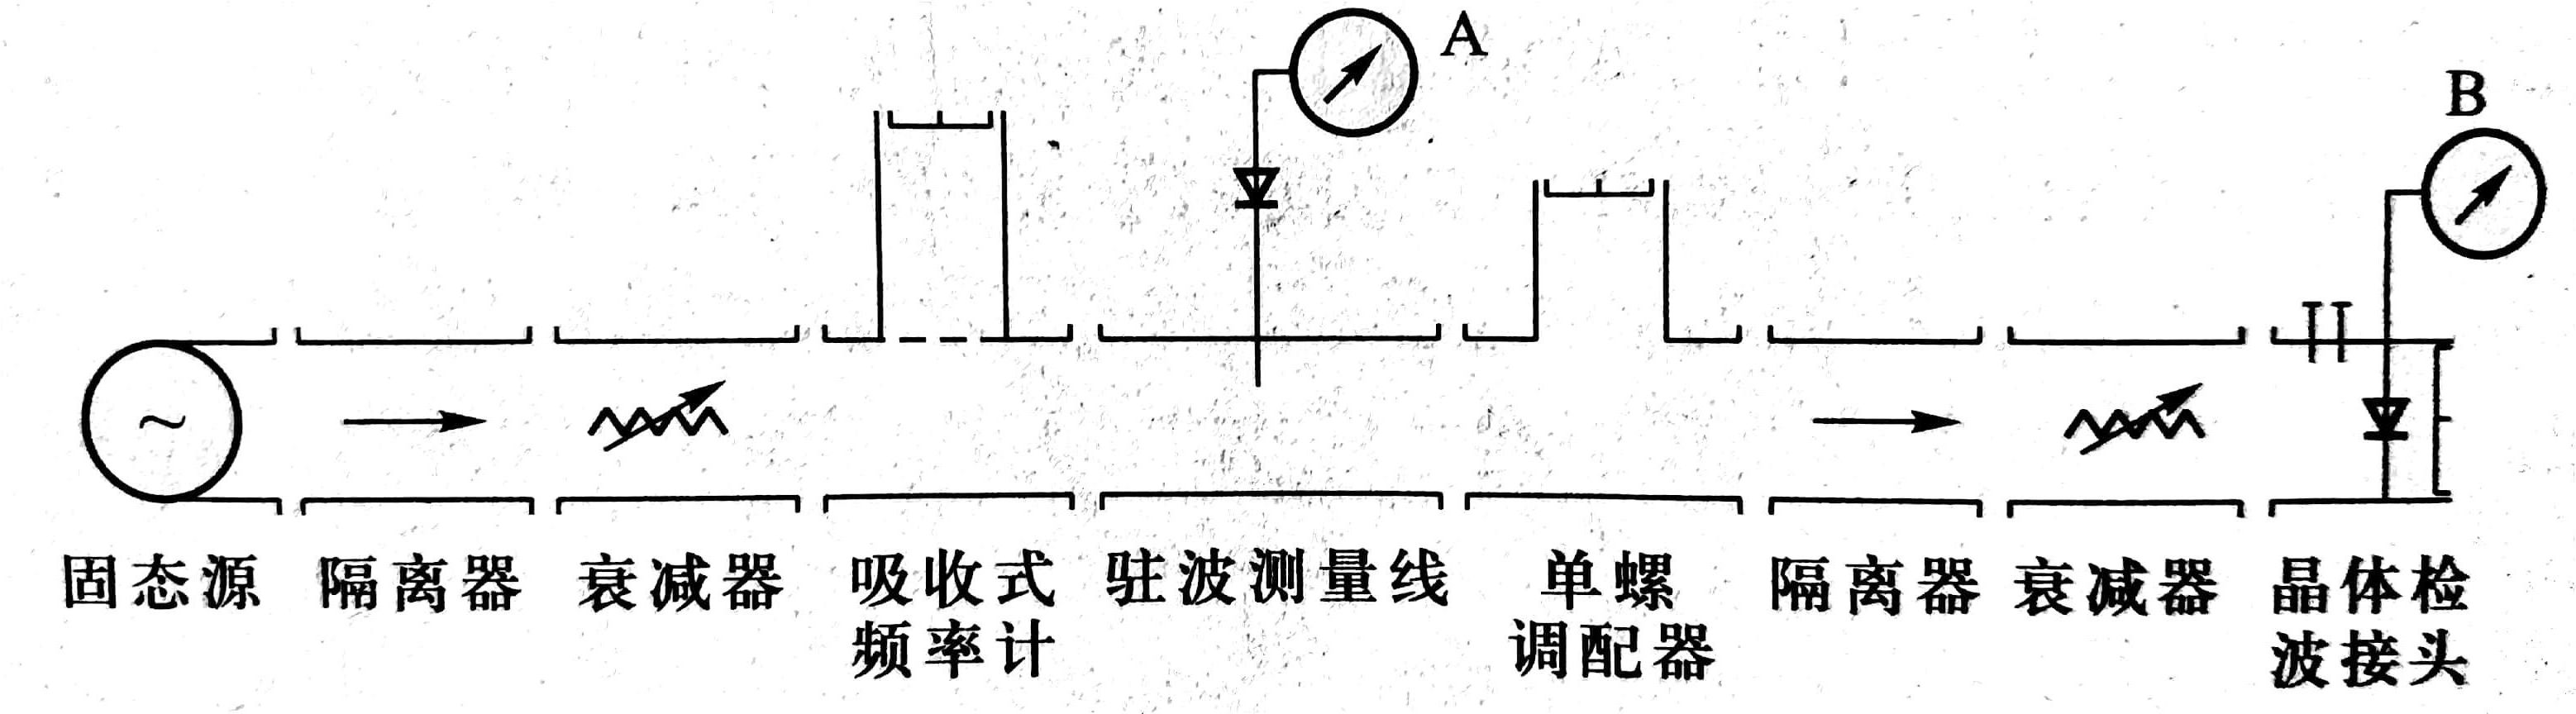
\includegraphics[width=100mm]{equip}
\caption{\label{fig:equip}%
康普顿散射实验装置图. 其中散射样品为铝棒($\phi=20\mathrm{mm}$)。放射源为一个约$10\mathrm{mCi}$的$\Cs$源,密封在铅室屏蔽体内;另有作能量刻度用的$^{60}\mathrm{Co}$放射源放在实验室储藏箱内,用时取出用胶带贴在探头口上。$\mathrm{NaI}$探测器能够以散射棒为中心转动(0 - 120$\degree$),与多道一体机相连。}
\end{figure}
本实验是由$\Cs$放射源出射$\gamma$光子,经准直孔打在实验台上的铝散射棒上,产生的散射光子用NaI闪烁谱仪接收,然后输出的脉冲信号,经线性放大器适当放大脉冲幅度,送到微机多道,测出散射光子的能谱。NaI探测器能够以散射棒为中心而转动,这样就能不断改变散射角$\theta$,测不同角度下的散射光子能谱。仪器装置见图~\ref{fig:equip}。

探头高压HV ADJ=520V,增益倍数调为0(使得$\Cs$的主峰位置在460道附近). 每次采集时间定为$10\mathrm{min}$。

\section{结果与讨论}
\subsection{通过$\Cs$和$\Co$的$\gamma$光子能谱定能量刻度}
半开$\Cs$源,在$0\degree$测量$\Cs$和$\Co$的$\gamma$光子能谱如图~\ref{fig:fig3}。
\begin{figure}[h]
\centering
\includegraphics[width=120mm]{03}
\caption{\label{fig:fig3}%
$\Cs$和$\Co$的$\gamma$光子能谱. $\Cs$峰在460道,道计数为26998;$\Co$两峰道址分别为817和934,道计数分别为5317和3853.}
\end{figure}

\begin{table}[h]
\caption{\label{tab:table1}%
测量$\Cs$和$\Co$出射$\gamma$光子的光电峰峰位定能量刻度. }
\begin{tabular}{|c|c|c|c|}
\hline
&$\Cs$&\multicolumn{2}{|c|}{$\Co$}\\\hline
能量/MeV&0.662&1.17&1.33\\\hline
道址\footnote{道址为固定单位:0 - 1024}&460&817&934\\\hline
\end{tabular}
\end{table}
\begin{figure}[h]
\centering
\includegraphics[width=120mm]{02}
\caption{\label{fig:fit}%
通过$\Cs$和$\Co$的$\gamma$光子能谱定能量刻度}
\end{figure}

用最小二乘法拟合直线,如图~\ref{fig:fit}所示。直线方程为
\begin{equation}
E=0.0014125 x + 0.012996 \label{eq:fit}
\end{equation}
(单位为MeV)。$R^2=0.99994$。可以认为探测器测量的道址与接收光子能量成很好的正比关系。定标完成后,我们将用式~\ref{eq:fit}来计算测得的道址所对应的光子能量。
\subsection{测量不同散射角$\theta$下的光子能谱,研究散射光子能量$E$和微分截面$\cs$与$\theta$的关系}
完全打开$\Cs$源,分别在$\theta$为$20\degree$, $40\degree$, $60\degree$, $80\degree$, $100\degree$, $120\degree$下测量$\Cs$经铝棒散射的光子能谱,记录峰的道址,峰下的总面积,测量到的光子能谱如图\ref{fig:07}。取下铝棒后测量每个角度下的本底谱(相同道数区间的本底面积)。测量得到的数据如表\ref{tab:stats}所示,与理论值的比较如表\ref{tab:contrast}所示。

从图\ref{fig:05}和图\ref{fig:06}可以看出,随着散射角$\theta$的增大,能量和散射截面都逐渐减小,总体趋势与理论预测时符合的。
\begin{table}[h]
\caption{\label{tab:stats}%
不同散射角$\theta$下的$\Cs$散射光子能谱}
\begin{tabular}{|c|c|c|c|c|c|c|}
\hline
角度$\theta$	&	$20\degree$	&	$40\degree$	&	$60\degree$	&	$80\degree$	&	$100\degree$	&	$120\degree$	\\\hline
道址	&	424	&	356	&	280	&	221	&	181	&	152	\\\hline
峰下总计数\footnote{峰的宽度:左右边界选在高度为峰值约1/3处}		&	28294	&	22321	&	17293	&	15319	&	15961	&	18173	\\\hline
本底计数\footnote{与上一行取相同的道数区间}	&	1209	&	744	&	632	&	659	&	741	&	1014	\\\hline
净散射计数	&	27085	&	21577	&	16661	&	14660	&	15220	&	17159	\\\hline
$E/\mathrm{keV}$\footnote{由式(\ref{eq:fit})得到}		&	611.891	&	515.842	&	408.493	&	325.156	&	268.657	&	227.694	\\\hline
$\eta \times 10 ^{-4}$\footnote{$\eta$和$R$在相应能量下的值可通过某些能量下的已知数据内插得到,见附录\ref{sec:interpolate}}	&	6.82	&	7.28	&	8.04	&	8.86	&	9.59	&	10.12	\\\hline
$R$	&	0.4196	&	0.4795	&	0.5777	&	0.6863	&	0.7722	&	0.8384	\\\hline
相对微分散射截面\footnote{取$\theta=20\degree$时的相对值为1,则可由式(\ref{eq:cs})得到}	&	1	&	0.653304	&	0.379163	&	0.254639	&	0.217185	&	0.213777	\\\hline
\end{tabular}
\end{table}
\begin{table}[h]
\caption{\label{tab:contrast}%
实测值与理论值对比}
\begin{tabular}{|c|c|c|c|c|c|c|}
\hline
$E_{th}/\mathrm{keV}$\footnote{式(\ref{eq:Eth})}	&	613.735	&	507.823	&	401.635	&	319.645	&	262.597	&	224.898	\\\hline
$E_{exp}/\mathrm{keV}$		&	611.891	&	515.842	&	408.493	&	325.156	&	268.657	&	227.694	\\\hline
相对误差$\times 100 \%$	&	-0.3	&	+1.6	&	+1.7	&	+1.7	&	+2.3	&	+1.2	\\\hline
相对微分截面, 理论值\footnote{式(\ref{eq:csth})}		&	1	&	0.598763	&	0.339499	&	0.226688	&0.188014	&	0.179363	\\\hline
相对微分截面, 实测值	&	1	&	0.653304	&	0.379163	&	0.254639	&	0.217185	&	0.213777	\\\hline
相对误差$\times 100 \%$	&	0	&	+9.1	&	+11.7	&	+12.3	&	+15.5	&	+19.2	\\\hline
\end{tabular}
\end{table}
\begin{figure}[h]
\centering
\includegraphics[width=120mm]{05}
\caption{\label{fig:05}%
对照散射$\gamma$光子的能量$E$的理论值与实测值}
\end{figure}
\begin{figure}[h]
\centering
\includegraphics[width=120mm]{06}
\caption{\label{fig:06}%
对照散射$\gamma$光子的微分截面$\cs$的理论值与实测值}
\end{figure}

将散射光子能量$E$的理论值与实测值对照作图如图\ref{fig:05}。从表\ref{tab:contrast}和图\ref{fig:05}中都可以看出能量$E$的实测值和理论值差距相当小。分析误差的主要来源可能是实际的角度有一定偏差;或者能量刻度不是完全准确。

将散射光子的微分截面$\cs$的理论值与实测值对照作图如图\ref{fig:06}。从表\ref{tab:contrast}和图\ref{fig:06}中都可以看出,相比于能量$E$,微分截面$\cs$的实测值与理论值的差距还是相当大的。而且散射角$\theta$越大,偏差越显著,$\theta=120\degree$时实测值与理论值的偏差达到了$+19.2\%$,而此时的本底计数只占总计数的不到6\%,说明即使考虑到无散射本底谱的影响后,还有很大的偏差。下面对微分截面的实测值和理论值不完全相符的原因予以解释:

首先,微分散射截面的定义中$\d \Omega$是一个无限小角度,而实验中探测器的立体角是有限大的,并用它来近似求微分散射截面。这样做可能会引入误差。从图\ref{fig:06}中的理论曲线可以看处,当$\theta$角较大时($\theta>80\degree$),$\cs$随$\theta$变化较缓慢,有限立体角对大角度几乎没有影响;但当$\theta$角较小时,$\cs$随$\theta$下降显著,导致探测器的有限立体角内测量出的平均微分散射截面偏小(凸函数性质),从而大角度下的微分散射截面的相对值就偏大。

然而我认为这仍不是偏差的主要来源。还应考虑环境散射的影响。虽然我们实验中扣除了本底,但环境散射的影响没法完全消除。由于仪器的布局问题,在散射角较大的情况下,探测器更容易额外接收到来自墙壁的散射粒子,使大角度情况下实验值偏大。此外,即使环境的附加计数为不依赖于角度的定值,大角度下的测量值本身偏小,相对误差就显得大了。

\begin{figure}[h]
\centering
\includegraphics[width=180mm]{07}
\caption{\label{fig:07}%
$\theta$为$20\degree$, $40\degree$, $60\degree$, $80\degree$, $100\degree$, $120\degree$下测量$\Cs$经铝棒散射的光子能谱}
\end{figure}

\section{结论}
本实验先用$\Cs$和$\Co$放射源在$0\degree$的光子能谱定能量刻度。然后分别测量了一系列散射角下的$\Cs$散射光子能谱和本底谱,计算得到了散射光子能量$E$和微分截面$\frac{\mathrm{d} \sigma}{\mathrm{d}\Omega}$与散射角$\theta$的关系,并于理论值比较,并尝试探讨了实验值和理论值不完全相符的原因。

\section{致谢}
感谢本次实验的指导老师付恩刚,细心地指导同学们放射性实验的注意事项。


\begin{thebibliography}{}
\bibitem{Book} 吴思诚, 荀坤 2015 近代物理实验(第四版)(北京:高等教育出版社).
\bibitem{Book} 赵凯华, 罗蔚茵 2001 新概念物理教程—量子物理 (北京:高等教育出版社)
\end{thebibliography}
\clearpage
\appendix
\section{思考题}
已在“结果于讨论”部分中回答
\section{作图插值求$\eta(\theta)$, $R(\theta)$}\label{sec:interpolate}
教材[2]第77页的表 2-4-1 和 2-4-2 给出了某些能量(如0.1, 0.2, 0.3, ... MeV)下$\eta$和$R$的取值,由此我们可以通过三次样条函数内插,近似得到 0.2 - 1.0 MeV 中每一能量对应的$\eta$和$R$,如图\ref{fig:interpolate}所示。
\begin{figure}[h]
\centering
\includegraphics[width=140mm]{04}
\caption{\label{fig:interpolate}%
样条插值求各能量$E$对应的$\eta$和$R$}
\end{figure}
\end{document}
